\documentclass[12pt]{article}
\usepackage[utf8]{inputenc}
\usepackage{graphicx}
\usepackage{listings}
\usepackage{lstautogobble}
\usepackage{amsmath} 
\usepackage[backend=bibtex]{biblatex}
\graphicspath{ {images/} }
\usepackage{float}
\floatstyle{boxed} 
\restylefloat{figure}
\usepackage{xfrac}

% Create struct diagrams
\usepackage{algorithm2e}
\SetAlgoLined
\SetKwProg{MyStruct}{Struct}{ contains}{end}

% Tikz directed graphs
% http://tex.stackexchange.com/questions/208947/how-can-i-draw-the-following-directed-graph
\usepackage{tikz}
\usetikzlibrary{positioning}

%\bibliographystyle{IEEEtran}
\bibliography{}
\AtEveryBibitem{%
  \clearfield{note}%
}

%%%%%%%%%%%%%%%%%%%%%%%%%%%%%%%%%%%%%%%%
\begin{document}

% Testing a structure
\begin{algorithm}[H]
\MyStruct{Node}{
  Node* parent\;
  int size\;
  \tcp{other stuff}
}
\end{algorithm}

% Testing a Tikz directed graph
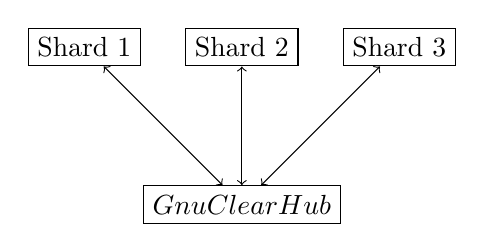
\begin{tikzpicture}
\pgfmathsetmacro{\shift}{0.25ex}
\node [draw] (1) at (0,2) {Shard 1};
\node [draw] (2) at (2,2) {Shard 2};
\node [draw] (3) at (4,2) {Shard 3};
\node [draw] (H) at (2,0) {$GnuClear Hub$};
\draw [<->] (1) -- (H);
\draw [<->] (2) -- (H);
\draw [<->] (3) -- (H);
%\draw [->,shorten <=-1pt, transform canvas={xshift=-\shift,yshift=-\shift}] (1) -- (3);
%\draw [->,shorten <=-1pt, transform canvas={xshift=\shift,yshift=\shift}] (3) -- (1);
\end{tikzpicture}

% Title
\title{
	{Ecclesia: A simple approach to self-organized public infrastructure}
}

\author{}
\date{\today}

\maketitle

\section{Introduction}

The combined success of the open-source ecosystem, of decentralized file-sharing, and of public cryptocurrencies,
has inspired an understanding that decentralized internet protocols 
can be used to radically improve socioeconomic infrastructure.
Such protocols provide a means of participation which is accessible, meaningful, and rewarding,
and a resulting service which is accountable and secure against malicious behaviour.

To date, however, networks implementing such protocols suffer from a number of drawbacks,
including their gross inefficiency, poor performance and scalability, difficulty to work with,
and the precarious legal condition of their access tokens.

Here, we present Ecclesia, a public network which simultanesouly addresses all of these problems.
Ecclesia uses Tendermint, which provides a high-performance, safe, secure consensus engine that is easy to scale, 
and where strict accountability guarantees hold over the behaviour of malicious actors.
At the application level, Ecclesia hosts a simple cryptocurrency and a formal governance mechanism enabling
the network to adapt and upgrade. 
The economics are designed with organic growth and sustainability in mind, 
and specifically avoids a single, large, upfront crowdsale.

We intend for Ecclesia to start simple, and to upgrade and/or fork over time 
according to the will and needs of its users.
That said, we conclude the paper with a potential roadmap.

\section{Tendermint}

In this section we describe the core consensus protocol,
how it can be extended to an atomic broadcast protocol,
and how to build applications that utilize the atomic broadcast.

\subsection{Consensus}

A fault tolerant consensus protocol enables a set of non-faulty processes
to eventually agree on a value proposed by at least one of them.
The problem is made more difficult by asynchronous network conditions,
wherein messages may have arbitrarily long delays, and by Byzantine faults,
wherein processes may exhibit arbitrary, possibly malicious, behavior.
In particular, it is well known that deterministic consensus in asynchronous networks in impossible \cite{flp},
and that consensus protocols can tolerate strictly fewer Byzantine faults than crash faults 
($\sfrac{1}{3}$ of processes, vs. $\sfrac{1}{2}$).
The former results from the inability to distinguish crash failures from asynchronous message delay.
The latter from the fact that three processes are not enough for a safe majority vote if one of them can lie (you need at least four).

In addition to providing optimal fault tolerance, a well designed consensus protocol
should provide additional guarantees in the event that the tolerance capacity is exceeded and the
consensus fails. This is especially necessary in public economic systems, 
where Byzantine behavior can have substantial financial reward. 
The most important such guarantee is a form of \emph{accountability},
where the processes that caused the consensus to fail can be identified and punished according to the rules of the protocol, or, possibly, the legal system.

Tendermint is a mostly asynchronous, optimally Byzantine consensus protocol, notable for its simplicity, performance, and accountability. We say mostly asynchronous because Tendermint employs a deterministic leader-based proposal mechanism,
thus incurring a weak synchrony assumption as faulty leaders must be detected and skipped.



security, accountability

\subsection{Atomic Broadcast}
consensus to atomic broadcast. why blocks. blockchain (this should be the only time we say blockchain!)

\subsection{Application Interface}
tmsp

\section{ Ecclesia }

The previous section described the core Tendermint algorithm
as it might be used in a traditional setting, to power, for instance,
an internet service offered by a corporation.
Using an atomic broadcast protocol in a public setting, however,
requires additional considerations, most particularly with regard to
spam prevention, incentive alignment, and governance.
In a private consensus environment, access is easily permissioned and rate-limitted,
and incentives are aligned by the formal structure of the legal entity maintaining the network (ie. a corporation).
In a public setting, the only known way to manage spam and align incentives is with the introduction of 
an explicit economics.

In this section, we describe the structure of the Ecclesia application,
which consists of two core modules: \emph{basecoin},  a generic multi-asset cryptocurrency;
and \emph{governmint}, a general purpose governance system that additionally enables collective administration of the validator set and of software upgrades.
Validators are required to post security deposits before they are eligible to be a validator,
such that if they are found to be malicious, their security deposit can be destroyed, 
or otherwise re-allocated according to governmint.

\subsection{ Basecoin }
describe basecoin

\subsection{ Governmint }
voting with tokens
changing validator sets
upgrades
forks

\section{ Distribution }
problem/importance of distribution
trouble with crowdsales
training, etc.
inflation

\section{Road Map}
shards, pegs, crypto
integrations
scalability

\section{Conclusion}



\printbibliography

\end{document}
